\part{Praktická část}

\hypertarget{analuxfdza-poux17eadavkux16f-na-aplikaci}{%
\chapter{Analýza požadavků na aplikaci}\label{analuxfdza-poux17eadavkux16f-na-aplikaci}}

V~praktické části této diplomové práce popisujeme výslednou webovou aplikaci pro geografické zmapování krajanských komunit a~jejich jazyka (dále jen aplikace). V~následujících kapitolách si ve stručnosti popíšeme související projekty, z~nichž jsme se při tvorbě více či méně inspirovali. Dále aplikaci představíme jak z~pohledu funkčních a~nefunkčních požadavků, tak z~hlediska návrhových a~implementačních částí.

\hypertarget{souvisejuxedcuxed-projekty}{%
\section{Související projekty}\label{souvisejuxedcuxed-projekty}}

XXX

\hypertarget{poux17eadavky-na-aplikaci}{%
\section{Požadavky na aplikaci}\label{poux17eadavky-na-aplikaci}}

Ještě před návrhovou fází vývoje je u~jakéhokoliv typu aplikace zapotřebí mít vyjasněny všechny požadavky, které jsou na daný systém kladeny. Tyto požadavky lze rozlišit na dva základny typy, a~to na funkční a~nefunkční.

\hypertarget{funkux10dnuxed-poux17eadavky}{%
\subsection{Funkční požadavky}\label{funkux10dnuxed-poux17eadavky}}

Funkční požadavky vyplývají z~účelu aplikace a~jsou typicky definované zákazníkem nebo jiným zadavatelem aplikace. Souvisí tak se základními funkcemi, akcemi a~aktivitami, jimiž by mělo digitální řešení disponovat pro řešení konkrétních problémů~\parencite{Gorton2006}.

Tyto požadavky můžeme u~naší webové aplikace pro větší přehlednost rozdělit do tří hlavních kategorií.

\hypertarget{geografickuxe1-reprezentace-ux10deskuxfdch-komunit-na-mapux11b}{%
\subsubsection{Geografická reprezentace českých komunit na mapě}\label{geografickuxe1-reprezentace-ux10deskuxfdch-komunit-na-mapux11b}}

Jedním z~nejdůležitějších nároků na aplikaci je vizualizace jednotlivých českých komunit po celém světě. Aplikace má tak disponovat samostatnou stránkou, v~rámci které budou dostupné mapové podklady celého světa. Na této mapě mají být pak prostřednictvím mapových vrstev vizualizovány konkrétní české enklávy. Pod mapovými vrstvami myslíme n-úhelníkové plochy, které mohou mít na mapě jakýkoliv tvar a~velikost podle potřeby vybrané komunity (geografická místa komunit v~aplikaci popisujeme jako lokality). Má být tak možné vizualizovat jak malé osady, tak celé regiony nebo státy -- vrstvy se též mohou jakýmkoliv způsobem překrývat.

Zapotřebí je také zahrnout základní funkční požadavky, které se pojí s~obsluhou mapové aplikace. Jde o~možnosti oddalování, a~přibližování pohledu (spolu s~navráceném do výchozí pozice), navigaci na mapě pomocí posouvání kurzoru klikání myší/dotykem anebo prostřednictvím minimapy zobrazující vždy širší kontext vybraného pohledu. Další důležitou mapovou funkcí je vyhledávání lokalit na mapě. Aplikace má umožňovat přiblížení na danou mapovou vrstvu na základě výběru ve vyhledávacím poli.

Zacílení lokalit má být umožněno i~jiným způsobem, než vyhledáváním v~mapových podkladech. Z~toho důvodu má aplikace disponovat výčtem lokalit, které budou dostupné z~mapové stránky prostřednictvím levé vysouvací části obrazovky. Tato sekce má sloužit jako přehledný abecedně seřazený seznam všech dostupných krajanských komunit (spolu s~úvodním obrázkem a~sekundárních názvem), z~něhož je možné lokalitu buď zacílit na mapě, anebo rovnou zobrazit její detail.

Posledním funkčním požadavkem souvisícím s~geografickou složkou je možnost filtrování lokalit na základě vybraných metrik (tyto metriky rozvedeme v~kapitole týkající se dat viz XXX). Tato funkce se má nacházet v~sekci se seřazenými komunitami a~po označení libovolného počtu filtrů se mají z~výběru i~z~mapových podkladů vyfiltrovat takové lokality, jež splňují danou podmínku.

\hypertarget{vizualizace-detailnuxedch-informacuxed-vybranuxe9-komunity}{%
\subsubsection{Vizualizace detailních informací vybrané komunity}\label{vizualizace-detailnuxedch-informacuxed-vybranuxe9-komunity}}

Druhým významným požadavkem na naši aplikaci je uživatelky přívětivá vizualizace všech dostupných informací, které se týkají vybrané krajanské komunity. Jelikož mohou být tyto informace rozličné velikosti a~multimediální povahy (audio soubory, obrázky, videa a~textové informace) je zapotřebí, aby v~aplikaci existoval sekundární navigační systém. Tato druhotná navigace má zajistit přehlednost při průchodu vybranou lokalitou a~umožnit tak uživateli výběr konkrétní části.

Jak bylo výše naznačeno, cílem našeho řešení je zmapovat ukázky komunikace v~češtině a~prostřednictvím audio nahrávek a~jejich transkriptů přiblížit jazyk dané české komunity. Požadavkem je tak také vhodné propojení audio souborů s~jejich přepisy.

Sekundárním požadavkem v~této oblasti je možnost sdílení vybrané lokality prostřednictvím URL adresy pro případnou kolaboraci při práci s~jednou určitou českou enklávou.

\hypertarget{administraux10dnuxed-prostux159eduxed-pro-editaci-jednotlivuxfdch-komunit}{%
\subsubsection{Administrační prostředí pro editaci jednotlivých komunit}\label{administraux10dnuxed-prostux159eduxed-pro-editaci-jednotlivuxfdch-komunit}}

Poslední kategorií jsou funkční požadavky spojené s~celkovou administrací jednotlivých komunit. Hlavní myšlenkou celé webové aplikace je otevřenost. A~to jak z~pohledu uživatele, který se chce dozvědět něco o~problematice (viz předchozí dvě kategorie), tak hlavně z~hlediska informované komunity, jež bude mít na starost přidávání nových lokalit, případě editaci či mazání již existujících oblastí.

Z~tohoto důvodu má aplikace obsahovat podstránky, které nebudou běžnému uživateli přístupné -- vzniká tak požadavek na autentifikaci prostřednictvím e-mailu a~hesla. Po úspěšném přihlášení by se měl celý systém přeměnit do editačního módu, respektive nabízet přihlášenému uživateli vždy kromě vstupu do jednotlivých lokalit i~možnost přesunu do administrativní části.

Ta by měla sestávat ze stejných sekcí, jako u~detailu vybrané komunity. Navíc by však by měla obsahovat uživatelsky přívětivou část formuláře podle formátu dané části informací (např. pro vkládání textových informací textový editor, pro vkládání souborů speciální komponentu). Druhotným požadavkem je pak základní validace vstupních data, tedy kontrola, že má každá lokalita vyplněný alespoň hlavní název a~geografická data pro zobrazení na mapě (viz xxx).

S~administrací tak nutně souvisí i~požadavek na persistenci dat, tzn. potřeba ukládat data na vzdálenou databázi, aby byly informace pro všechny uživatele konzistentní a~aktualizované.

\hypertarget{nefunkux10dnuxed-poux17eadavky}{%
\subsection{Nefunkční požadavky}\label{nefunkux10dnuxed-poux17eadavky}}

Pod nefunkčními požadavky si lze představit určitá omezení na design a~implementaci aplikace. Zde se jedná například o~volbu technologií, míru bezpečnosti, důraz na výkon či udržitelnost do budoucna atd. V~závěru se však vždy jedná o~určitý kompromis napříč jednotlivými faktory (např. vysoký výkon vs.~udržitelnost)~\parencite{Gorton2006}.

Hlavním nefunkčním požadavkem je, aby byl náš systém realizován jako multiplatformní webová aplikace, protože lze tak efektivně docílit multiplatformnímu řešení. Z~tohoto faktu vyplývá potřeba responzivního řešení, tedy aby byla aplikace stejně funkční a~vzhledově atraktivní jak na zařízeních s~vyšším rozlišením, tak i~na menších obrazovkách. Dalším implicitním požadavkem je tím pádem i~nutnost internetového připojení.

Důležitou vlastností aplikace by také měla být udržitelnost a~škálovatelnost. V~tuto chvíli již existují konkrétní plány na rozšiřování aplikace mimo rozsah této diplomové práce, a~proto by měla být aplikace napsána se zásadami čistého a~čitelného kódu pro případné navázání jinými programátory.

Výběr technologií taktéž souvisí s~nefunkčními požadavky. Protože se jedná o~webovou aplikaci, její základ bude postaven na základních webových technologiích, jimiž jsou JavaScript, HTML a~CSS. Pro tvorbu uživatelského rozhraní bude zvolen javaScriptový framework React spolu s~využitím TypeScriptu a~pro autentifikaci a~databázové řešení bude vybrána platforma Firebase.

\hypertarget{nuxe1vrh-aplikace}{%
\chapter{Návrh aplikace}\label{nuxe1vrh-aplikace}}

V~rámci popisu návrhu se zaměříme na čtyři klíčová témata, jejichž obsah vychází především z~funkčních požadavků definovaných výše.

V~první části si představíme použité technologie spolu s~odůvodněním jejich výběru. V~další podkapitole popíšeme data, se kterými v~aplikaci pracujeme a~jakým způsobem je v~systému reprezentujeme.

Hlavní součástí této kapitoly pak bude představení uživatelského rozhraní prostřednictvím jednotlivých obrazovek aplikace. Zaměříme se zde také na popis interakce uživatele se systémem. Na závěr charakterizujeme základní architekturu aplikace.

\hypertarget{pouux17eituxe9-technologie}{%
\section{Použité technologie}\label{pouux17eituxe9-technologie}}

Jelikož je naše navrhované řešení webovou aplikací, budeme se níže zabývat výhradně nástroji, knihovnami a~frameworky, které se primárně týkají webových technologií.

\hypertarget{zuxe1kladnuxed-webovuxe9-technologie}{%
\subsection{Základní webové technologie}\label{zuxe1kladnuxed-webovuxe9-technologie}}

I~přes to, že je svět webových technologií jednou z~nejdynamičtěji rozvíjejících se oblastí IT, jeho základy jsou již několik desítek let stále stejné. Aby mohl webový prohlížeč vykreslit webovou stránku\footnote{Pojmy webová stránka a~webová aplikace vnímáme v~tomto kontextu totožně. Tedy vše, co platí pro vývoj webových stránek, platí i~pro vývoj webových aplikací (protože aplikace jsou v~principu jen komplexnější formou webových stránek).}, musí být její obsah vždy určitým způsobem strukturovaný. Pro tyto účely se již řadu let využívá HTML (Hypertext Markup Language) -- značkovací jazyk, který popisuje přesnou strukturu určitého dokumentu.

Prostřednictvím značek tohoto jazyka dáváme jednotlivým částem dokumentu strukturální významy. Mohou to být například značky pro označení odstavce, odkazů nebo třeba tabulek či videí. Některé značky sice mohou vyvolat změny vzhledu dané části dokumentu, nicméně pro tyto účely HTML není primárně určeno~\parencite{htmlcss}.

Abychom mohli upravit vzhled webové stránky, je zapotřebí využít druhé základní technologie, a~to CSS (Cascading Style Sheets). Jedná se o~jazyk, pomocí kterého lze konkrétním HTML značkám přiřazovat předdefinované vlastnosti, a~tak jim měnit vzhled dle potřeb. Typicky může jít o~změny barvy, velikosti, fontů, ale i~třeba o~implementaci složitějších animací, přechodů atd.~\parencite{htmlcss}.

HTML a~CSS lze od sebe izolovat do dvou či více separátních souborů, což je standardní způsob jak efektivně oddělit vizuální složku od strukturální.

Třetí základní technologií je programovací jazyk JavaScript (oficiálně ECMAscript), který předchozí dvě složky doplňuje o~možnost interakce uživatele s~webovou stránkou. JavaScript je skriptovací jazyk, který není narozdíl od jiných programovacích jazyků typu Java nebo Objective-C zapotřebí před spuštěním kompilovat (stačí tedy pro jeho použití využít jakýkoliv z~dostupných webových prohlížečů). Díky této technologii lze dynamicky upravovat obsah webové stránky, to znamená že JavaScript využijeme především v~situacích, kdy od uživatele očekáváme nějakou aktivitu (např. stisknutí tlačítka nebo klávesy atd.)~\parencite{javascript}.

Aby JavaScript a~CSS mohly přistupovat k~jednotlivým částem HTML, dochází vždy před vykreslením k~převedení ze značkovacího jazyka do takzvaného DOM (Document Object Model). Jedná se o~objekt stromové struktury, v~němž je uložené vlastní HTML a~každá značka (uzel) si drží informaci o~své lokaci. CSS pak na tento objekt aplikuje svá pravidla pro správné vykreslení a~JavaScript případně mění strukturu spolu s~další části tohoto stromového objektu~\parencite{howbrowserswork}.

\hypertarget{vykreslovuxe1nuxed-webovuxfdch-struxe1nek}{%
\subsection{Vykreslování webových stránek}\label{vykreslovuxe1nuxed-webovuxfdch-struxe1nek}}

Při výběru dalších technologií pro vývoj webové aplikace si je zapotřebí nejdříve uvědomit, jakou strategii vykreslování bude naše aplikace naplňovat.

\hypertarget{dynamickuxe9-webovuxe9-struxe1nky}{%
\subsubsection{Dynamické webové stránky}\label{dynamickuxe9-webovuxe9-struxe1nky}}

Jednou z~nejčastějších strategií je dynamické vykreslování stránek. Jedná se o~princip, kdy je webová stránka (tedy HTML s~CSS a~JavaScriptem) se všemi potřebnými informacemi dynamicky vytvořena na vzdáleném serveru. Prohlížeč (jinými slovy klient) tak na základě akce od uživatele pošle na server takzvaný \emph{request} a~server vygenerovanou webovou stránku obratem pošle nazpět.

Výhodou toho přístupu je fakt, že klient dostane už kompletní dokument se všemi potřebnými informacemi (což je výhodné z~hlediska SEO\footnote{Search engine optimization (SEO) je proces optimalizace viditelnosti webových stránek v~rámci internetových vyhledávačů jako je např. Google. Čím lepší je SEO, tím je pravděpodobnější, že se daná webová stránka objeví na vyšších příčkách při vyhledávání.}). Neméně důležitým přínosem je pak to, že se veškerá logika děje na serveru (který je typicky výkonnější než klient, prohlížeč akorát vykresluje výsledek.

Na druhou stranu lze vidět i~nevýhodu primárně v~opakovaném generování každé stránky při opětovné návštěvě, což může být problém při pomalejším internetovém připojení. Komplikovanější též může být vývoj samotných aplikací, protože vývojář musí znát jak HTML, CSS a~JavaScript (souhrnně frontend), tak technologie spojené se serverovou částí (práce s~databází atd.). protože jsou na sebe obě složky na serveru nutně navázané~\parencite{spa}.

\begin{figure}[ht]   
    \centering
    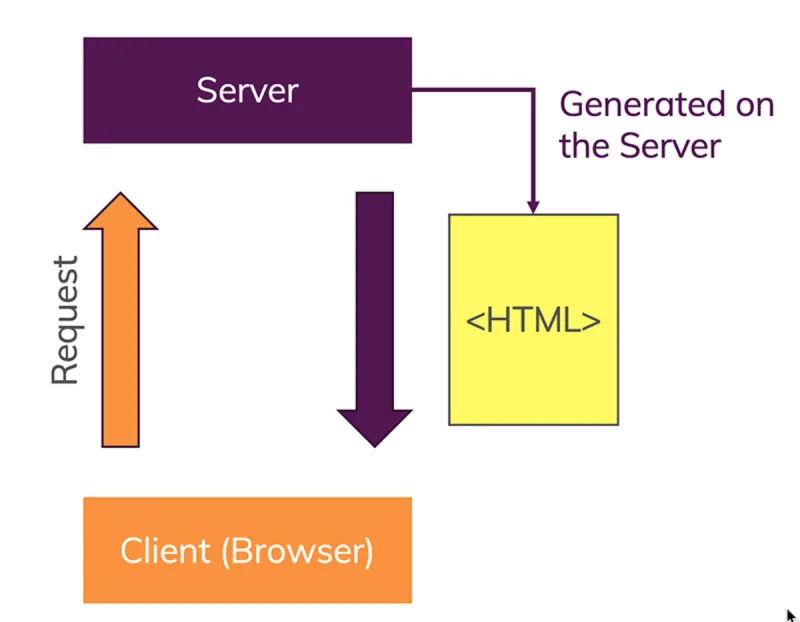
\includegraphics[width=.5\textwidth]{dynamic}  
    \caption{Dynamické vykreslování}
    \label{dynamic}
 \end{figure}

\hypertarget{statickuxe9-webovuxe9-struxe1nky}{%
\subsubsection{Statické webové stránky}\label{statickuxe9-webovuxe9-struxe1nky}}

Druhý přístup je nejstarší a~zároveň nejjednodušší, protože se jedná o~již vytvořené HTML (spolu s~CSS a~JavaScriptem) soubory, které jsou neměnné. To znamená, že jsou tyto již připravené statické soubory uložené na serveru, kde očekávají request od klienta k~vykreslení. Jedná se tedy nejčastěji o~takové webové stránky, které jsou jednodušší a~neočekává se u~nich příliš mnoho interaktivity s~uživatelem.

V~dnešní době jsou navíc populární takzvané generátory statických stránek, které umožňují vytvářet statické stránky na základě předpřipravených šablon a~odlehčeného značkovacího jazyka jako je například Markdown\footnote{[https://www.markdownguide.org/](https://www.markdownguide.org/)}, v~němž se vytváří samostatný obsah~\parencite{spa}.

\begin{figure}[ht]   
    \centering
    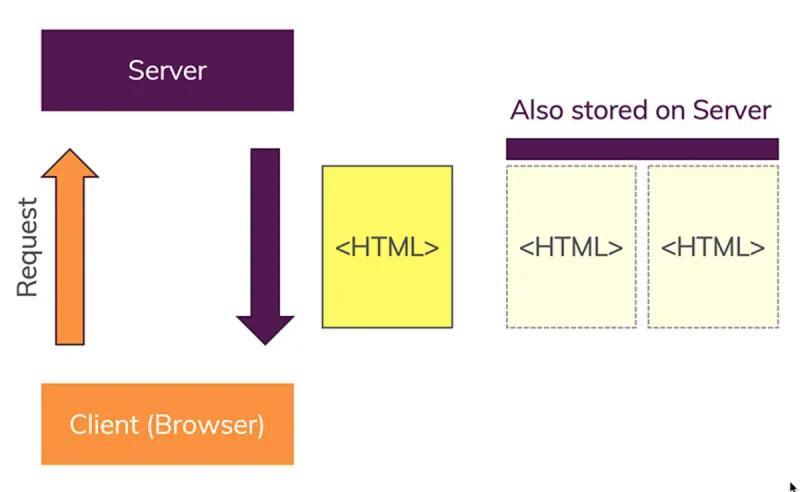
\includegraphics[width=.5\textwidth]{static}  
    \caption{Statické vykreslování}
    \label{static}
 \end{figure}
